	\newpage
\section{Testowanie}	%5
%Opisujemy testy, sprawdzamy czy nie generuje błędów.

\subsection{Włączenie aplikacji}
\newpage

\begin{figure}[H]
	\centering
	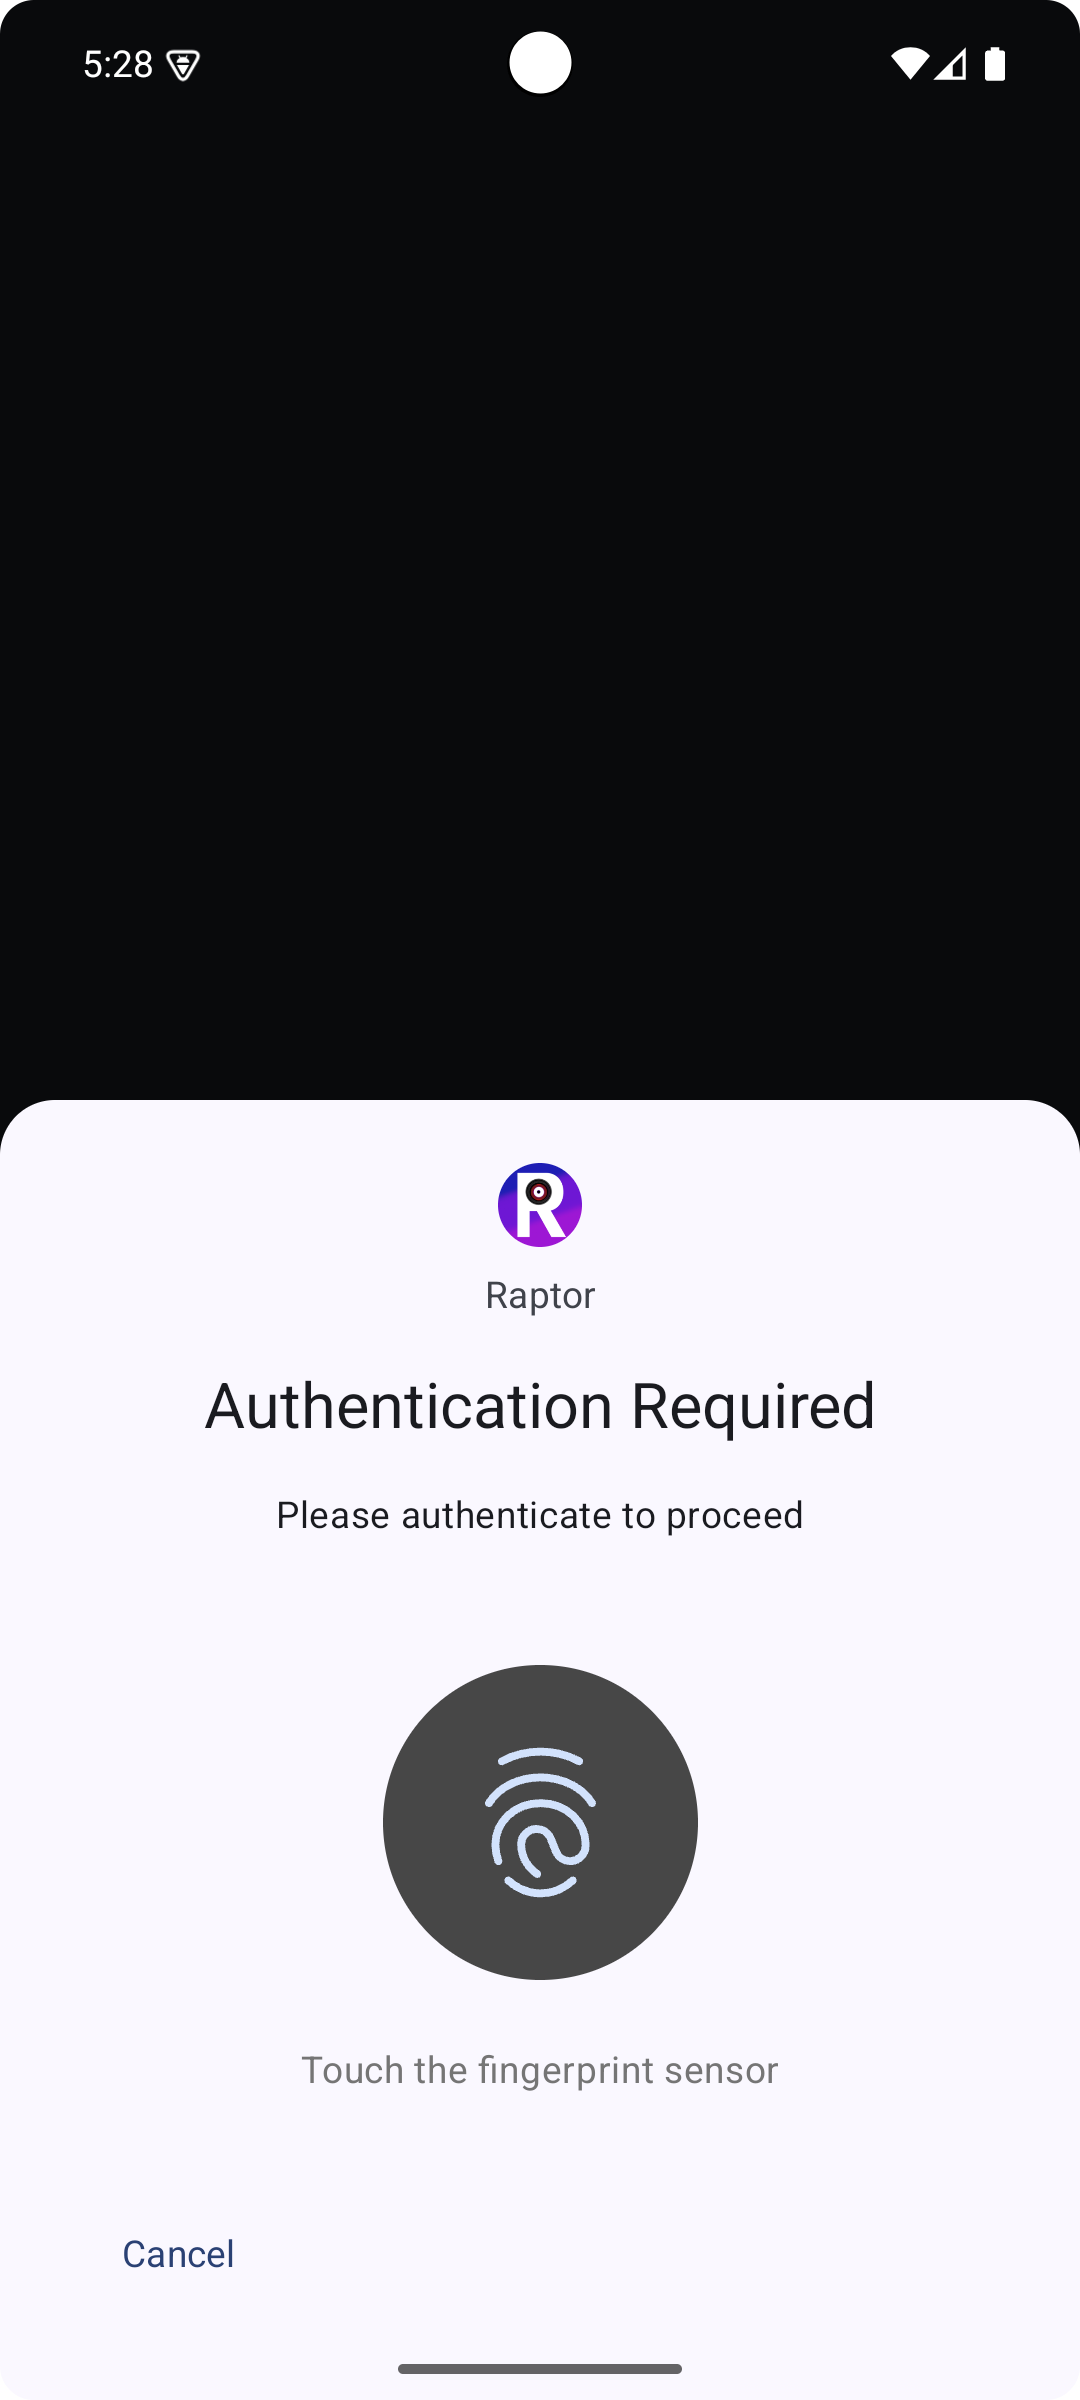
\includegraphics[width=1\textwidth]{images/usage_fingerprint.png}
	\caption{\centering{Prośba o podanie odcisku palca.}}
	\label{fig:test_fingerprint}
\end{figure}

\begin{figure}[H]
	\centering
	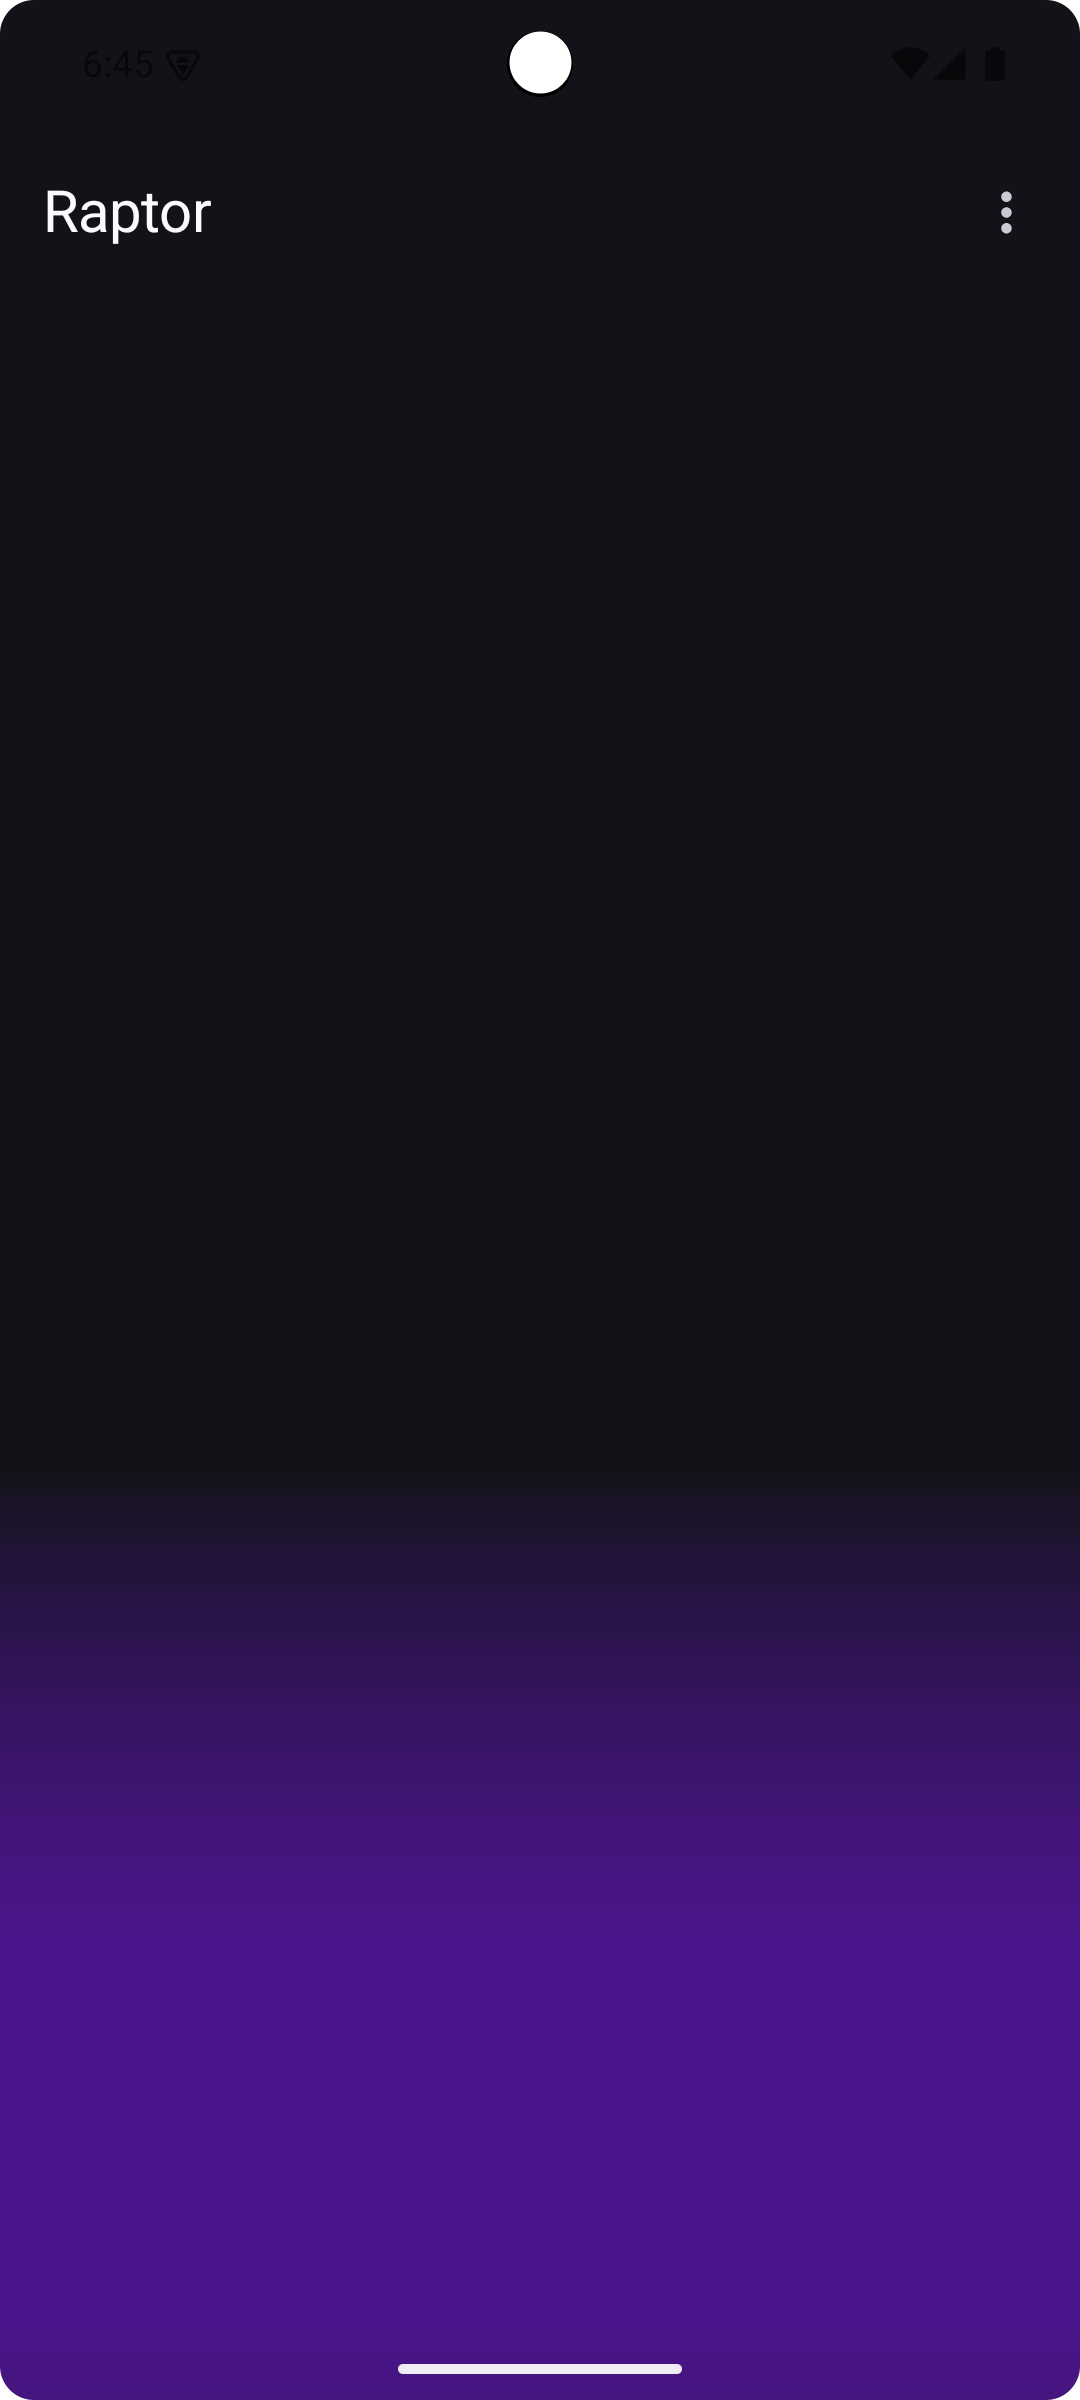
\includegraphics[width=1\textwidth]{images/tutorial_autorzy_pusty.png}
	\caption{\centering{Widok po zweryfikowaniu odcisku.}}
	\label{fig:test_autorzy_pusty}
\end{figure}

Zgodnie z założeniami, po otwarciu aplikacji pojawia się prośba o podanie odcisku palca (rysunek nr.~\ref{fig:test_fingerprint}). Po zweryfikowaniu, aplikacja pomyślnie przechodzi do głównego ekranu, jak pokazano na rysunku nr.~\ref{fig:test_autorzy_pusty}.

\subsection{Dodawanie utworów}

\begin{figure}[H]
	\centering
	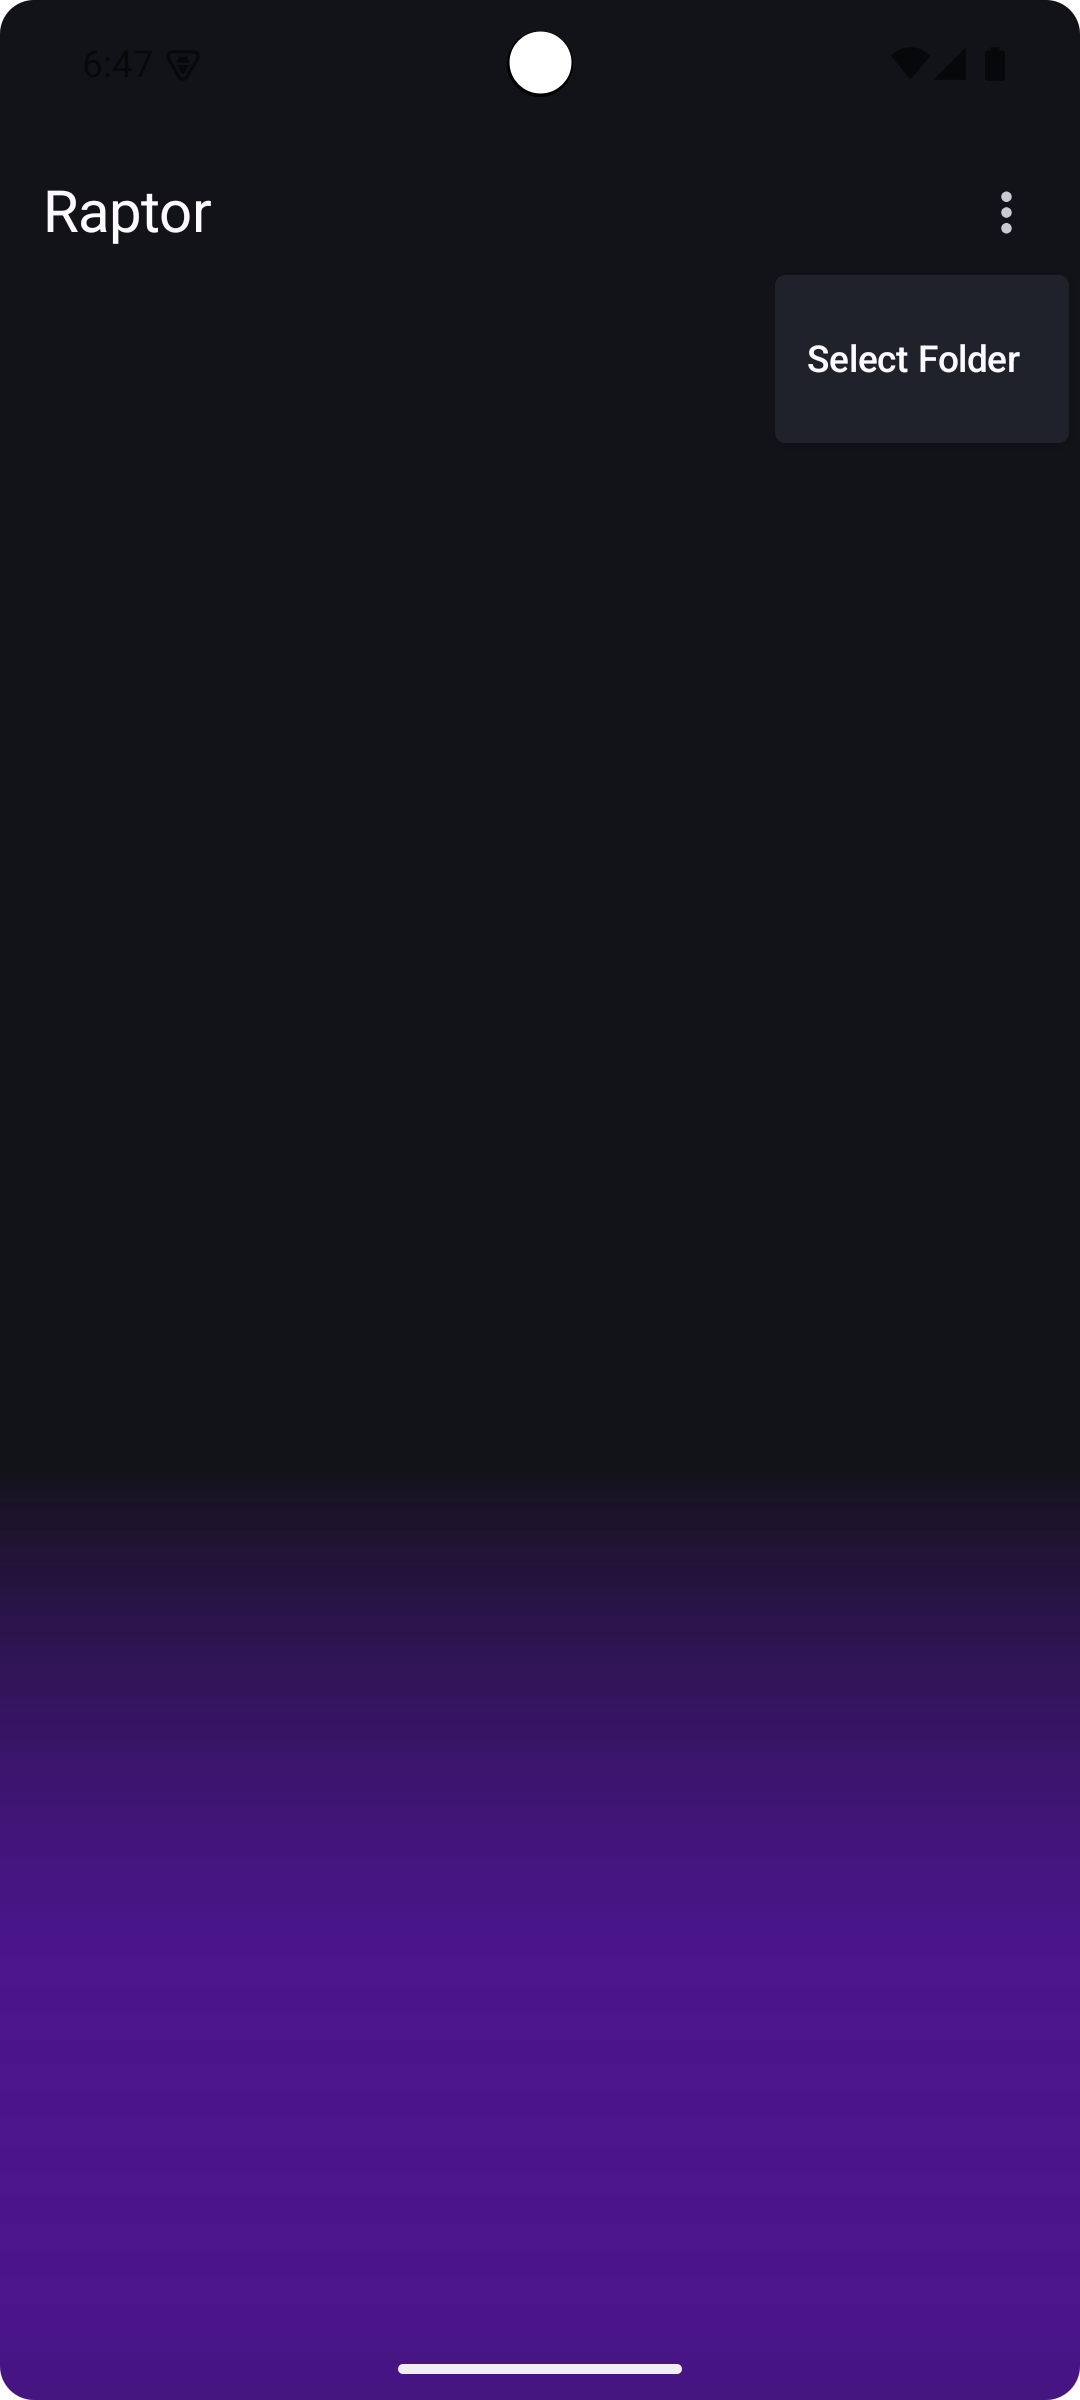
\includegraphics[width=1\textwidth]{images/tutorial_select_folder.png}
	\caption{\centering{Włączenie wyboru folderu.}}
	\label{fig:test_select_folder}
\end{figure}

\begin{figure}[H]
	\centering
	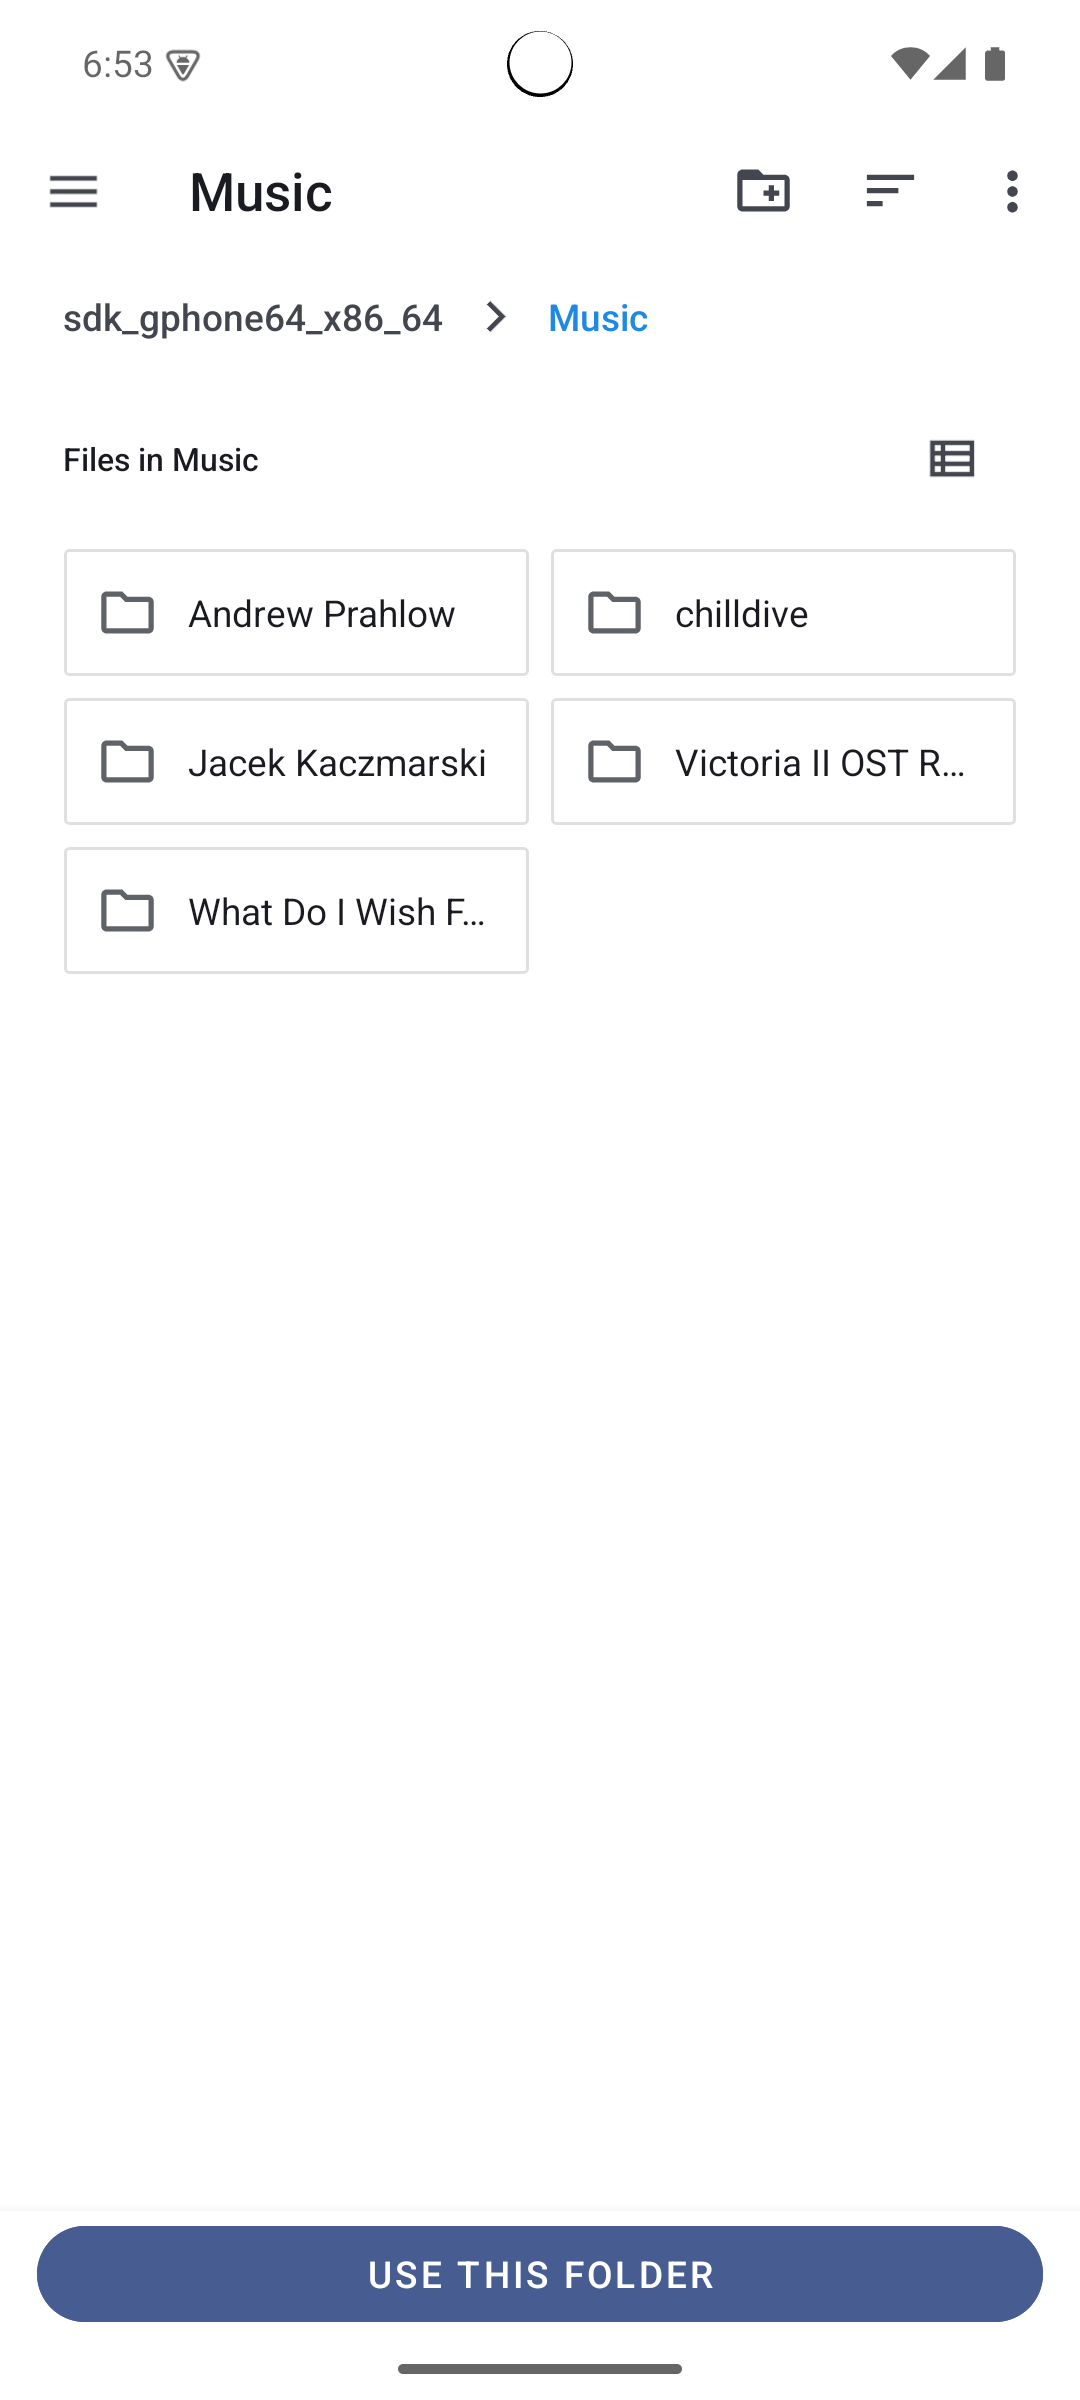
\includegraphics[width=1\textwidth]{images/tutorial_folder_selected.png}
	\caption{\centering{Wybieranie folderu z muzyką.}}
	\label{fig:test_folder_selected}
\end{figure}

\begin{figure}[H]
	\centering
	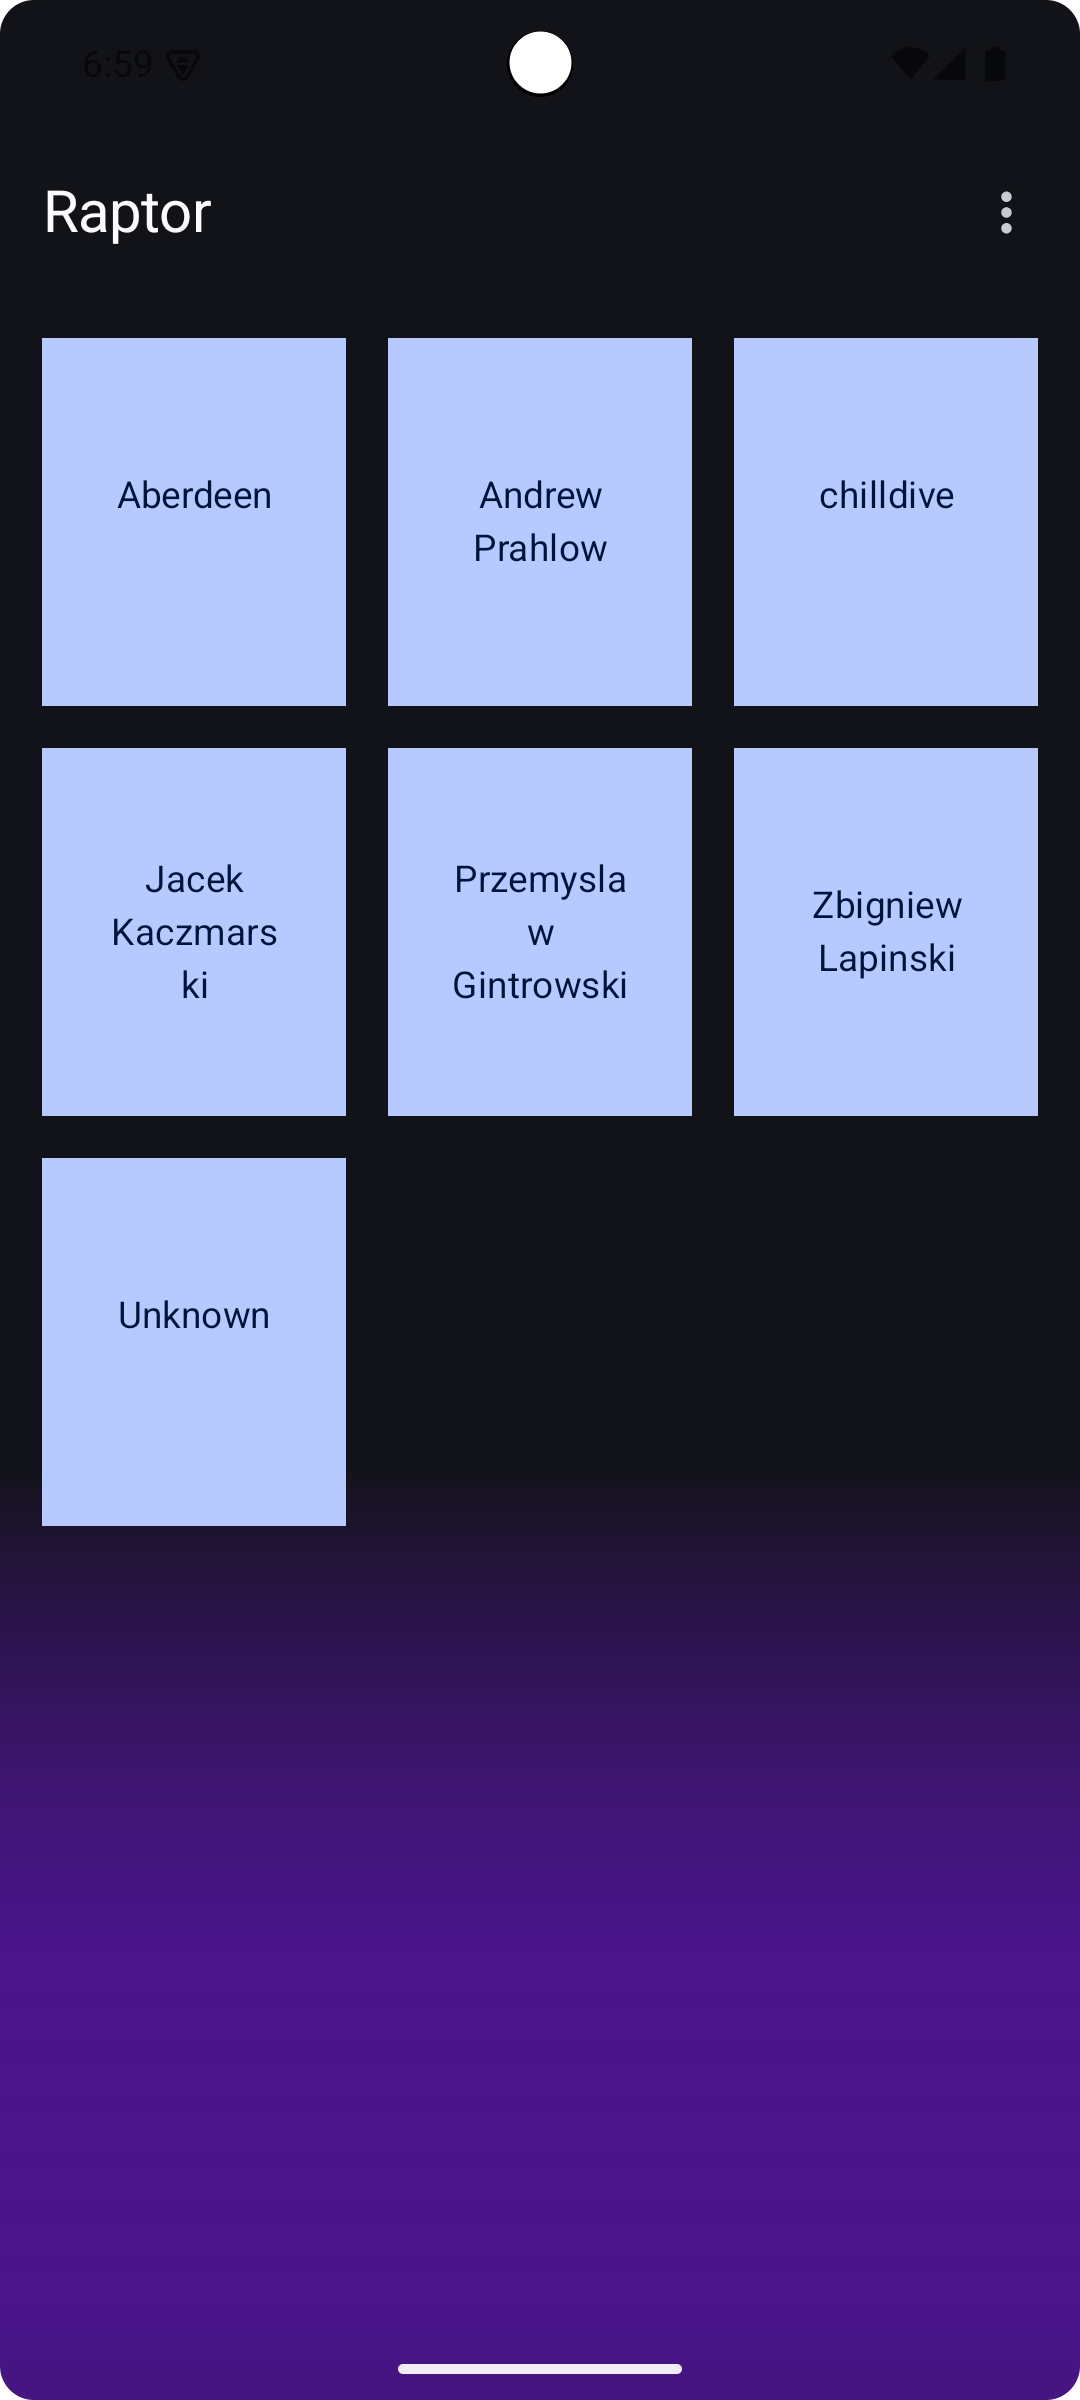
\includegraphics[width=1\textwidth]{images/tutorial_after_loading.png}
	\caption{\centering{Widok po załadowaniu plików.}}
	\label{fig:test_after_loading}
\end{figure}

Na rysunkach nr. \ref{fig:test_select_folder}, \ref{fig:test_folder_selected} i \ref{fig:test_after_loading} ukazana jest procedura ładowania plików piosenek. Jak widać piosenki załadowały się pomyślnie i interfejs odpowiednio reaguje na te zmiany. W kafelku o nawie \enquote{Unknown}, zawarte są piosenki bez otagowanego wykonawcy.

\subsection{Nawigacja}

\begin{figure}[H]
	\centering
	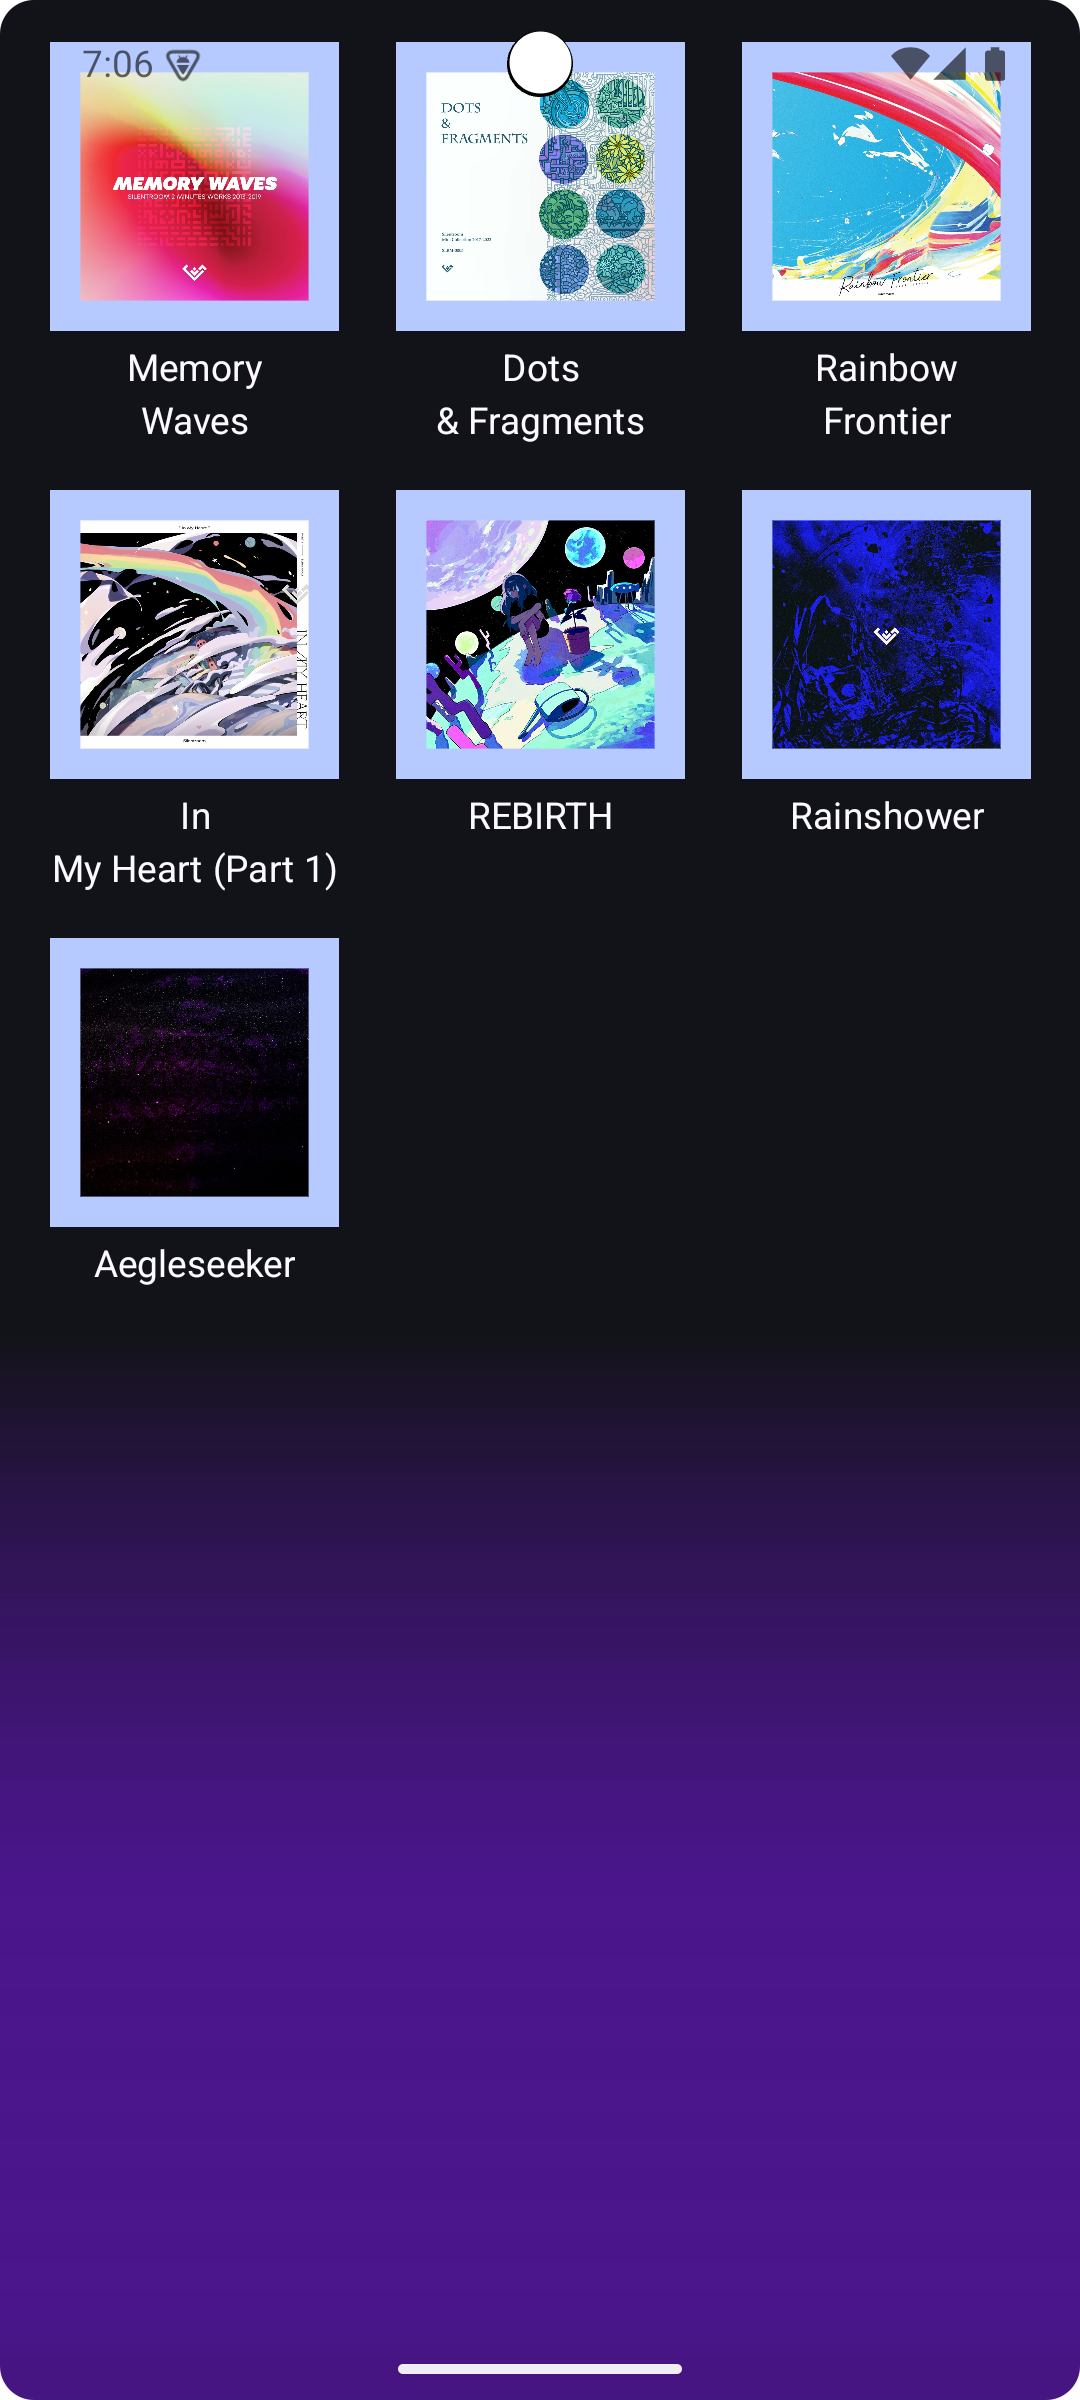
\includegraphics[width=1\textwidth]{images/tutorial_album_view.png}
	\caption{\centering{Widok po wejściu w autora.}}
	\label{fig:test_album_view}
\end{figure}

\begin{figure}[H]
	\centering
	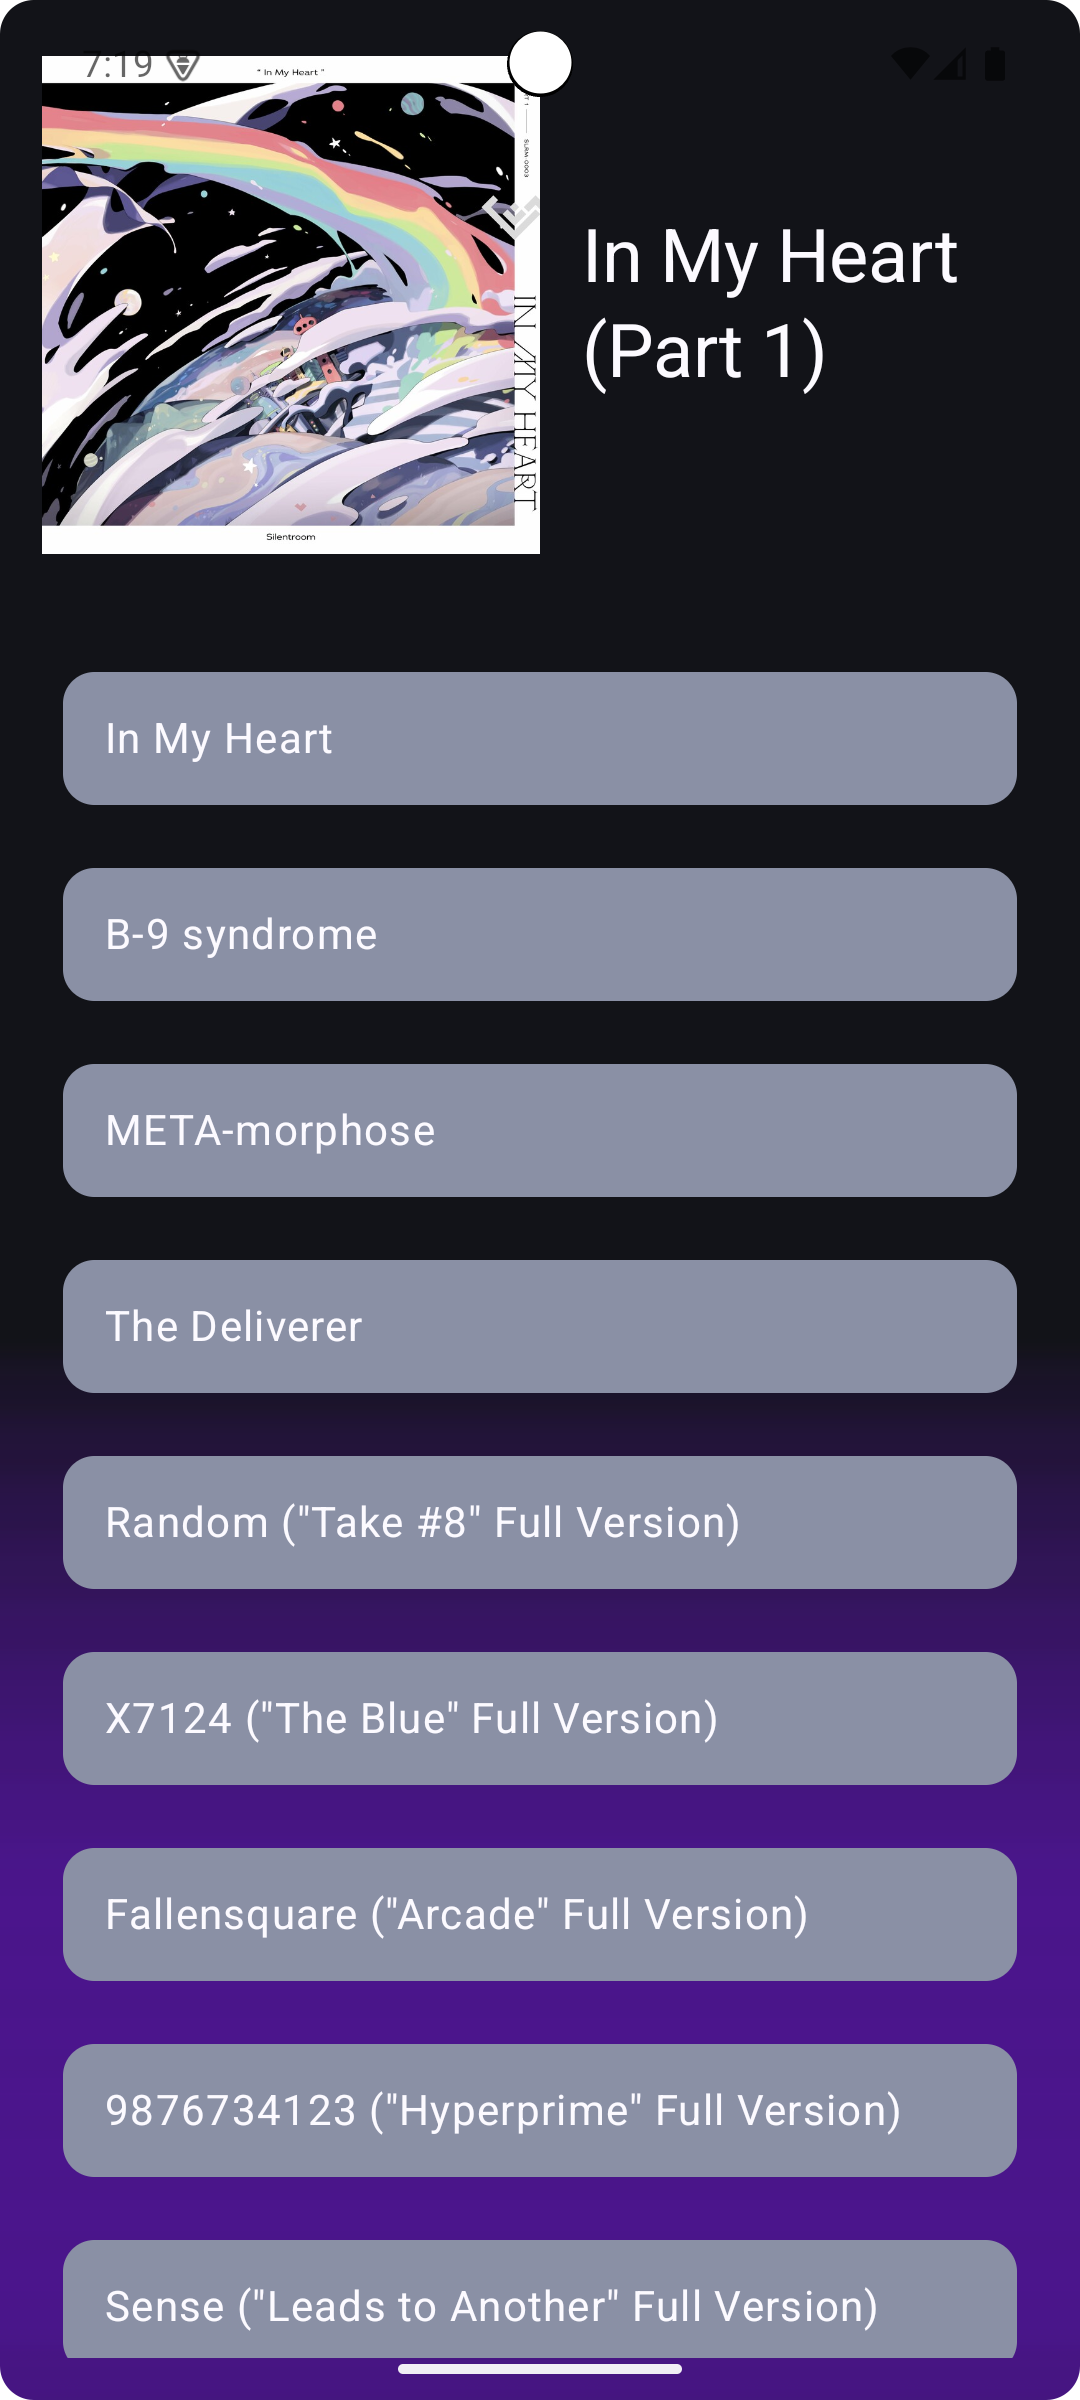
\includegraphics[width=1\textwidth]{images/tutorial_song_view.png}
	\caption{\centering{Widok wyboru piosenki.}}
	\label{fig:test_song_view}
\end{figure}

Na rysunku nr.~\ref{fig:test_album_view} pokazano, że pomyślnie można przejść do ekranu widoku albumów. Pomyślnie wyświetlają się wszystkie miniaturki. Analogicznie, z rys. nr.~\ref{fig:test_song_view} wynika, że można przejść do widoku piosenek. Podobnie, informacje o albumie, w którym są piosenki wyświetlają się pomyślnie. 

\subsection{Działanie odtwarzacza}

\begin{figure}[H]
	\centering
	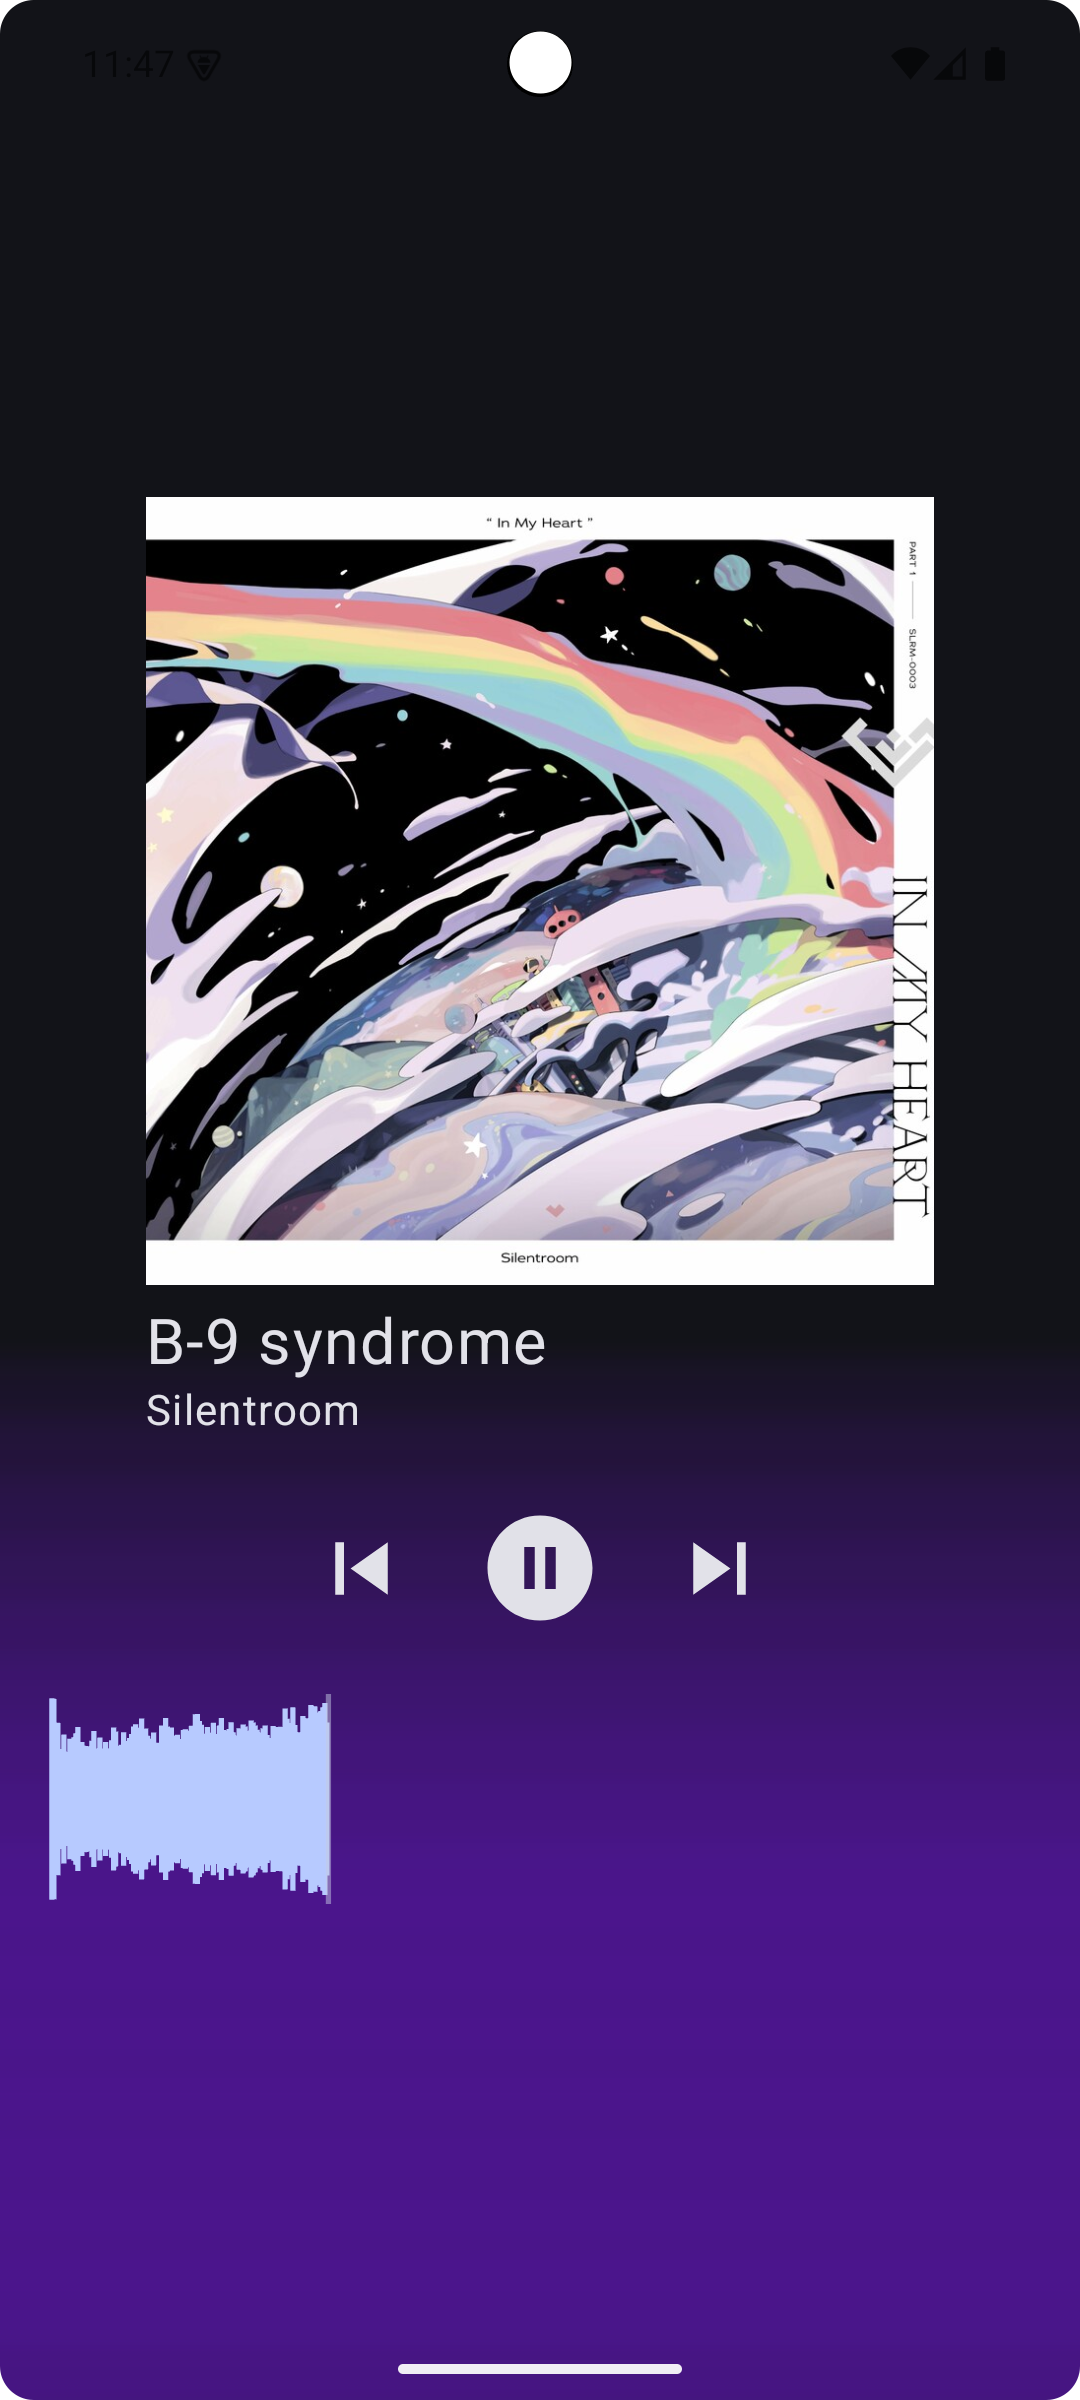
\includegraphics[width=1\textwidth]{images/test_player_playing.png}
	\caption{\centering{Odtwarzacz odgrywa piosenkę.}}
	\label{fig:test_player_playing}
\end{figure}

\begin{figure}[H]
	\centering
	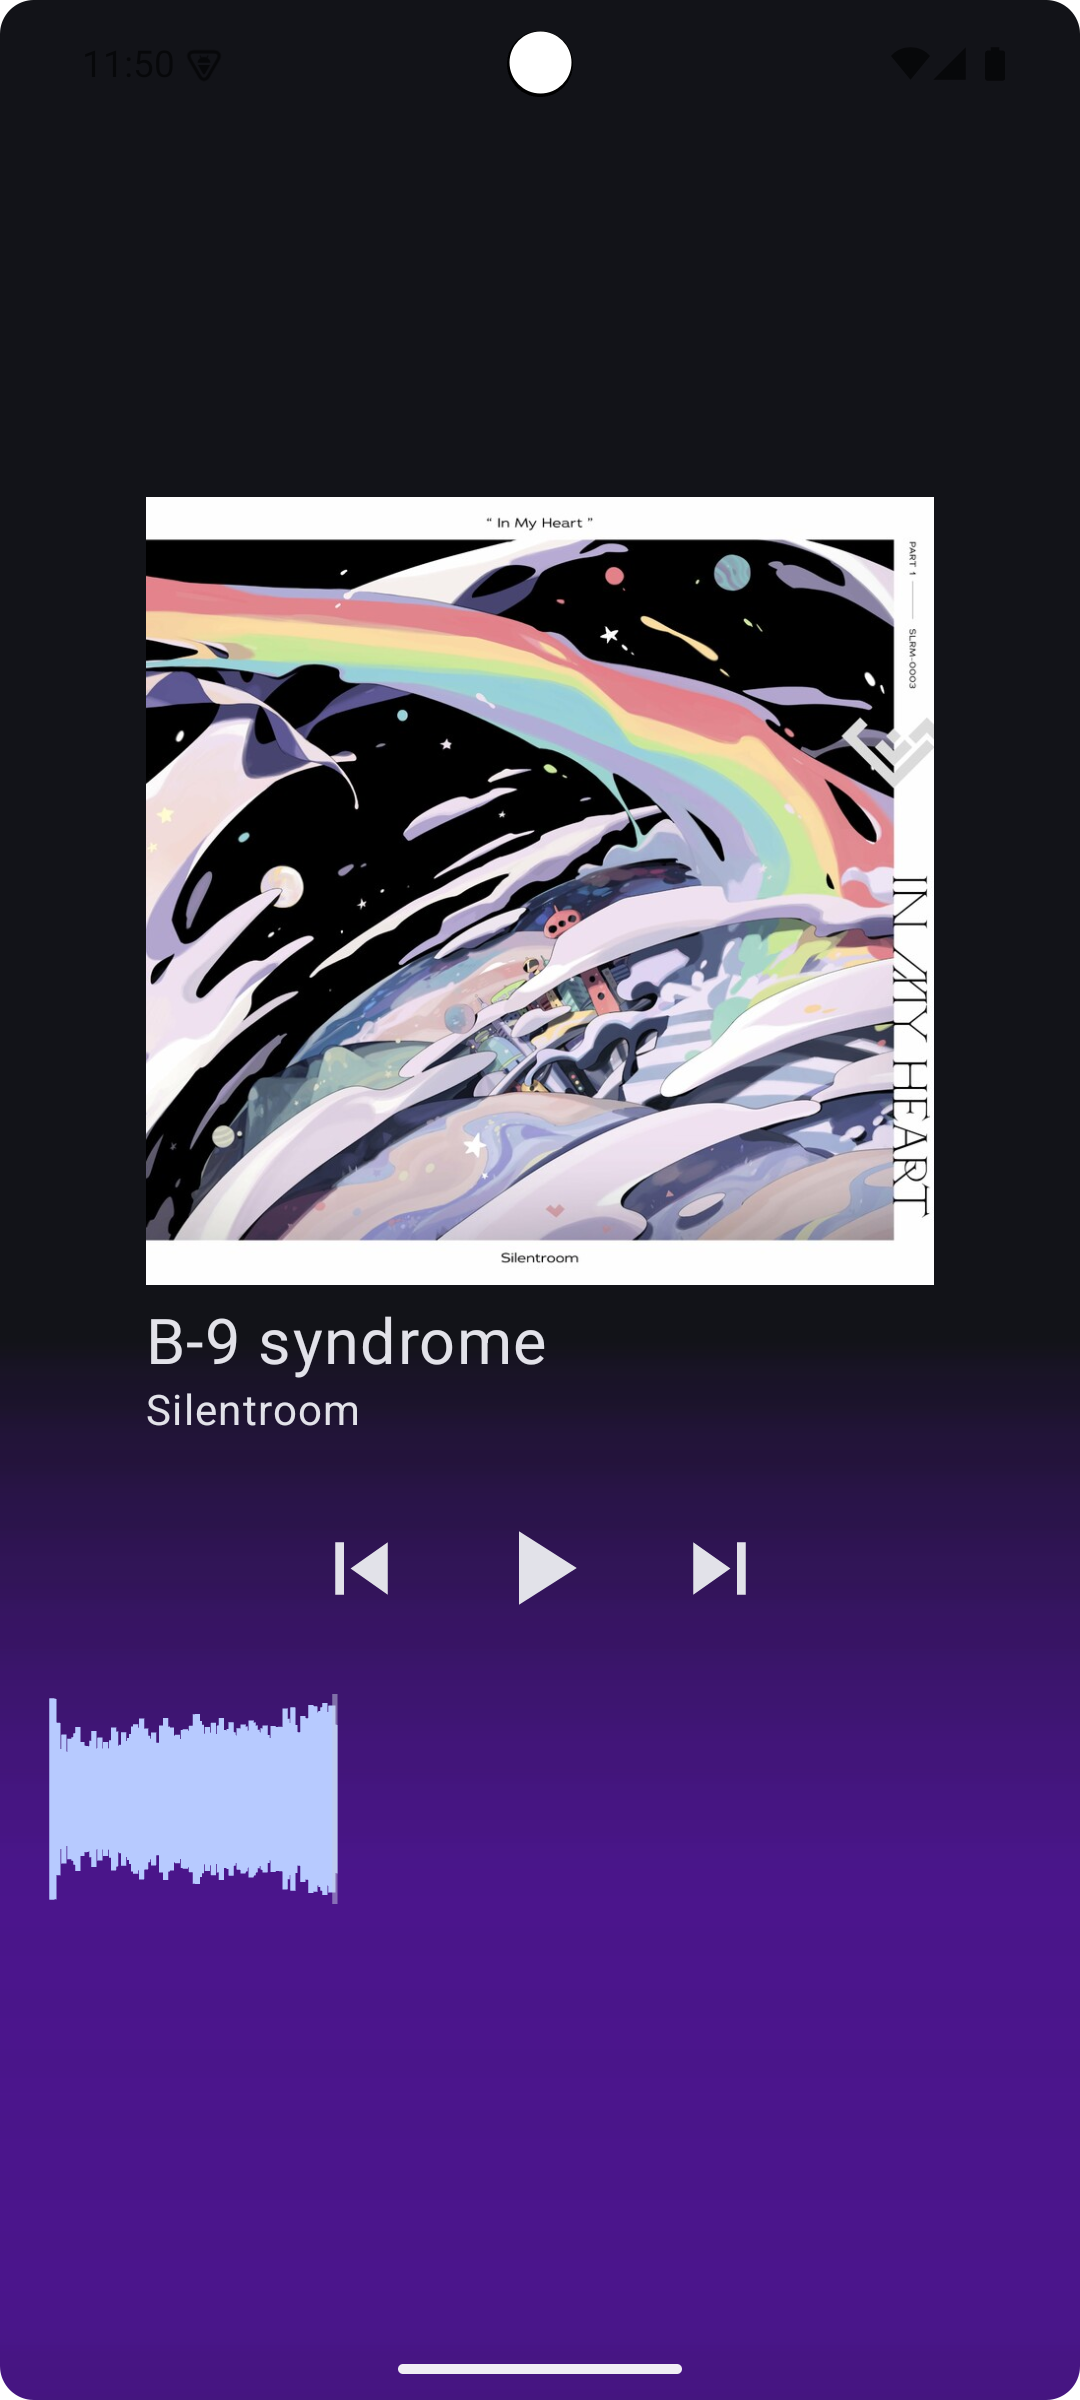
\includegraphics[width=1\textwidth]{images/test_player_paused.png}
	\caption{\centering{Piosenka w odtwarzaczu jest zapauzowana.}}
	\label{fig:test_player_paused}
\end{figure}

\begin{figure}[H]
	\centering
	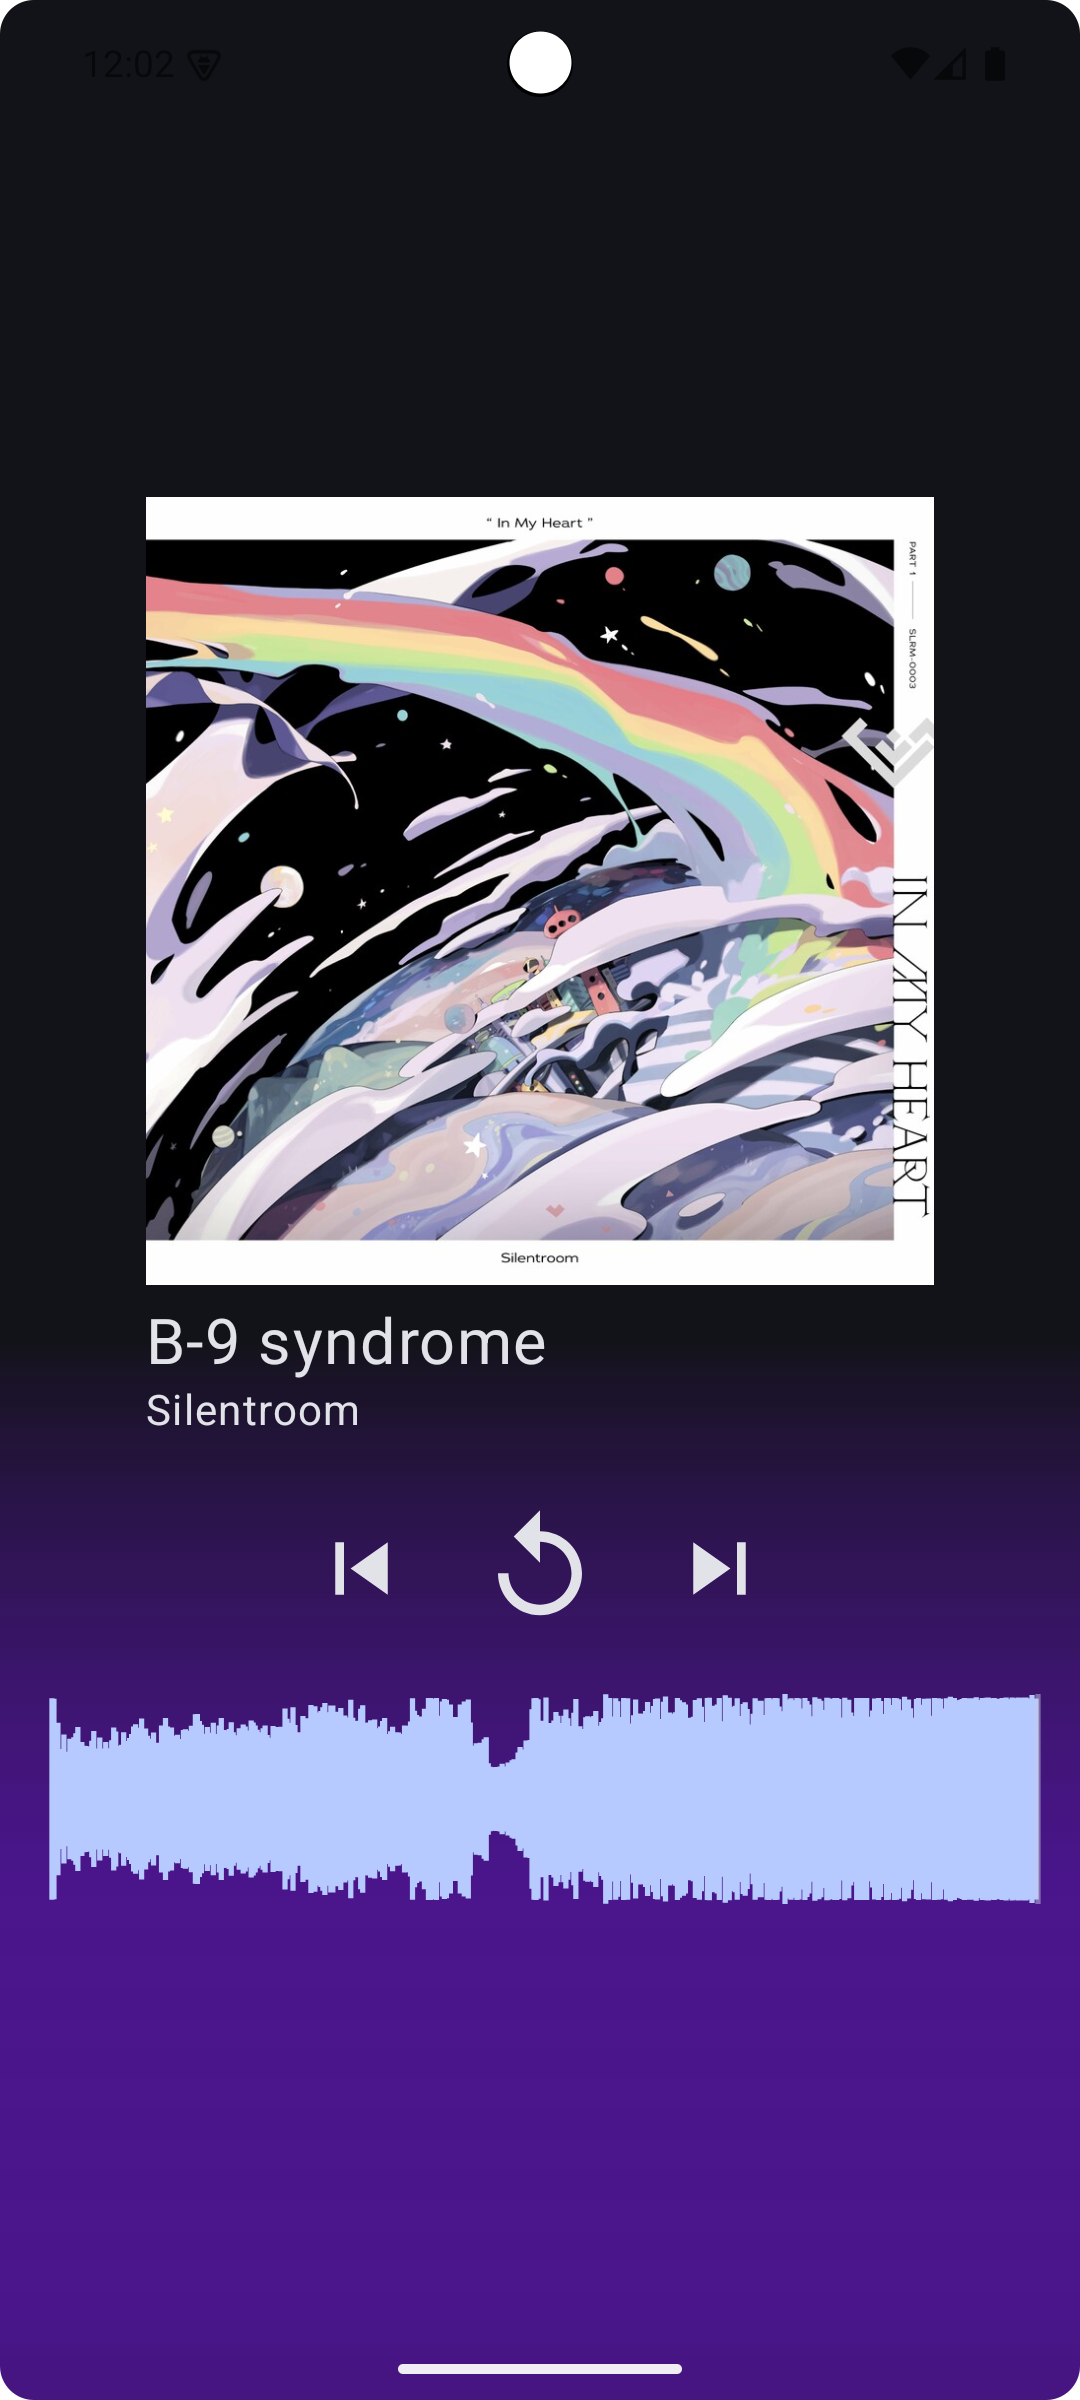
\includegraphics[width=1\textwidth]{images/test_player_stopped.png}
	\caption{\centering{Zatrzymany odtwarzacz}}
	\label{fig:test_player_stopped}
\end{figure}

Jak widać na rysunku nr.~\ref{fig:test_player_playing}, odtwarzacz pomyślnie odgrywa piosenkę. Z wiadomych przyczyn, trudno jest pokazać to, że słychać dźwięk. Ponadto pokazana jest miniaturka, generowany jest waverform oraz wyświetlane są informacje o piosence, mianowicie tytuł oraz wykonawcy. Na rysunku nr.~\ref{fig:test_player_paused}, pokazano, że odtwarzacz może być zapauzowany. Przeciągając progress bar do końca, można zauważyć, że pojawia się możliwość zrestartowania utworu.

\begin{figure}[H]
	\centering
	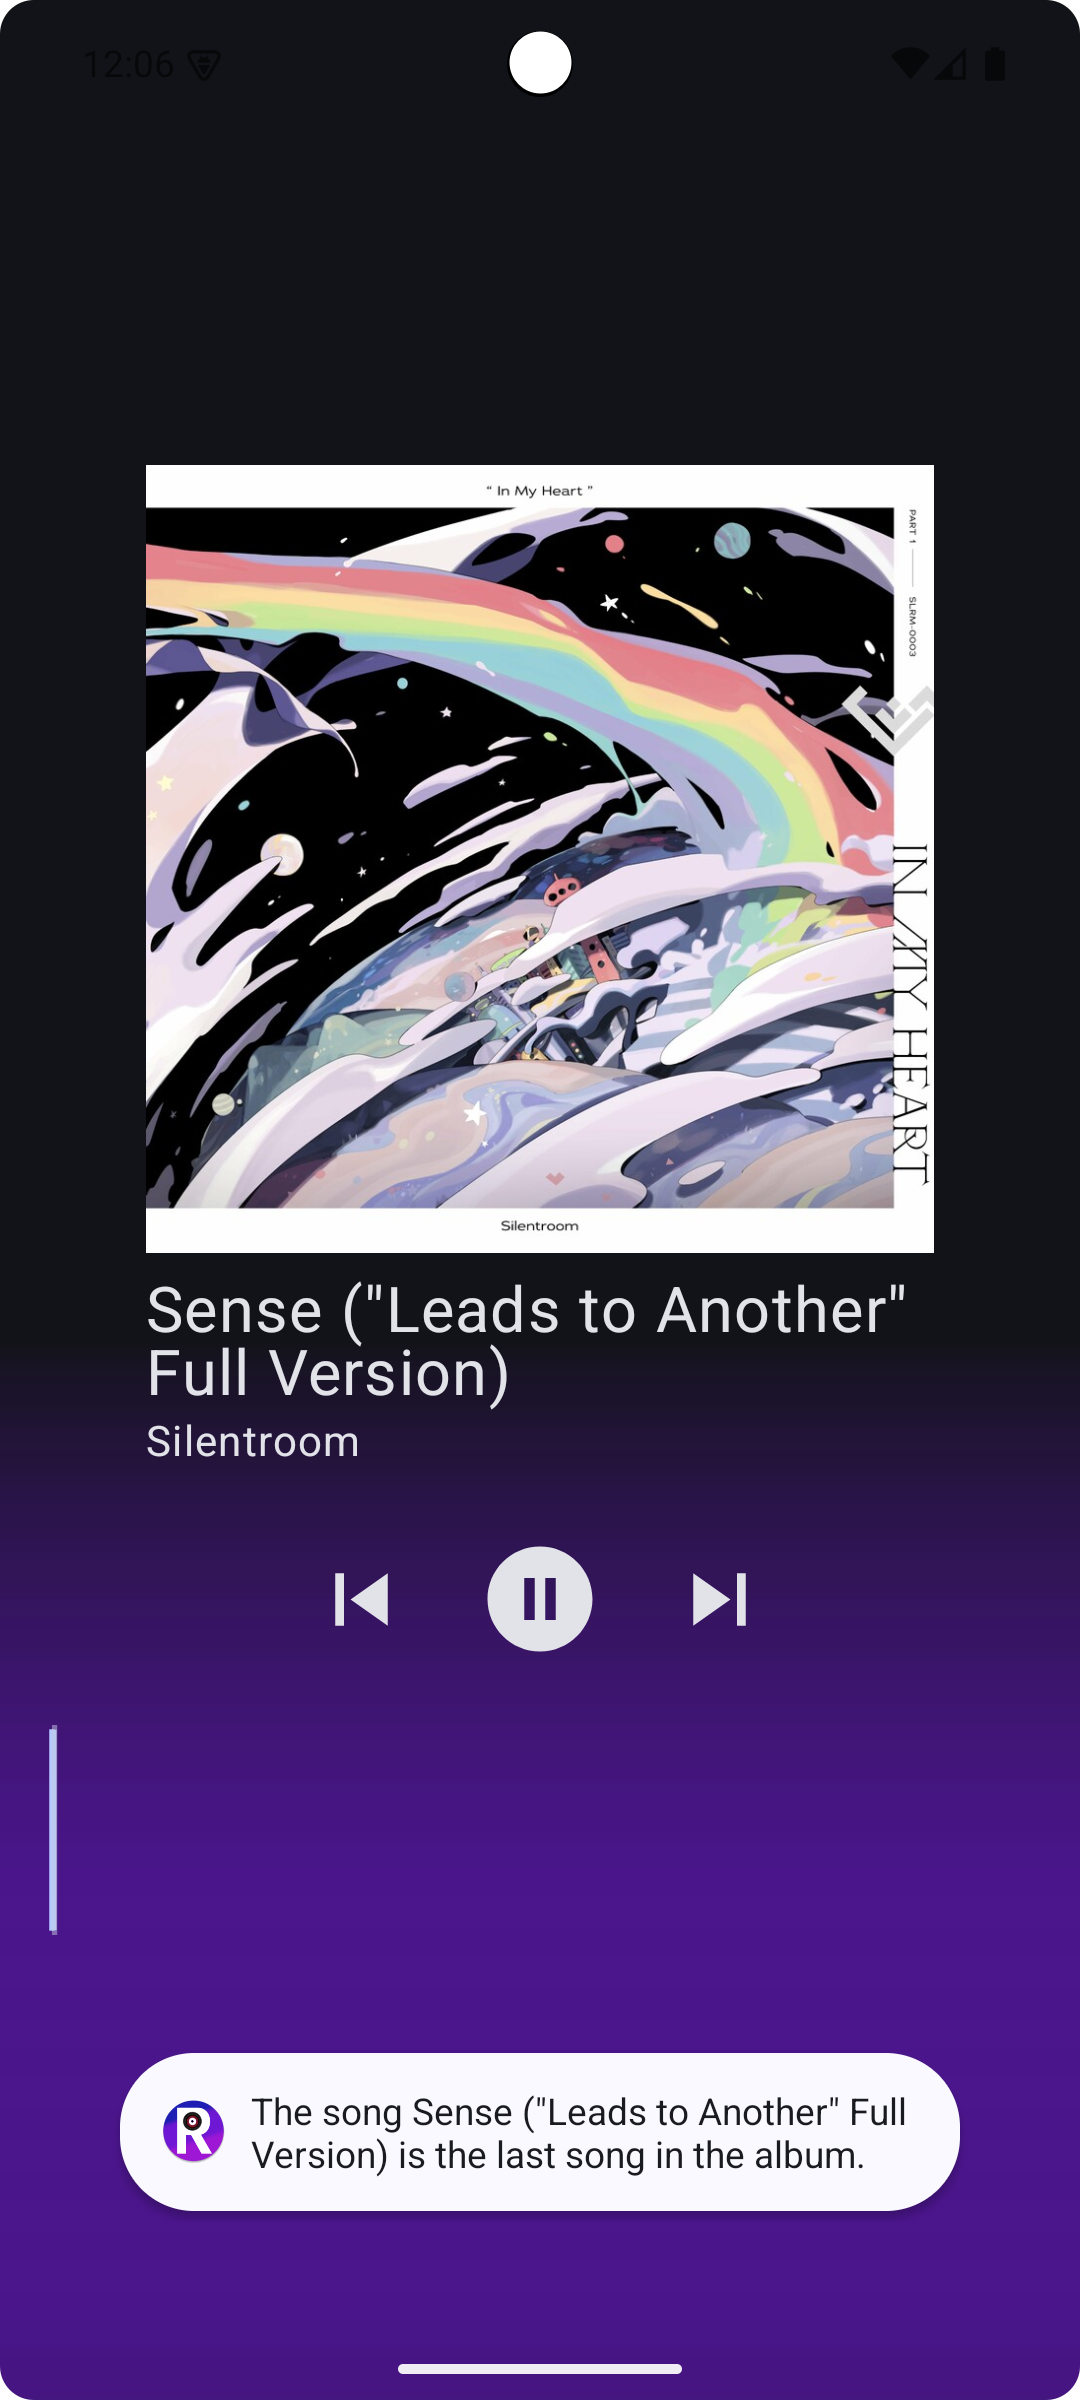
\includegraphics[width=1\textwidth]{images/test_player_nextcap.png}
	\caption{\centering{Przechodzenie przez album do końca}}
	\label{fig:test_player_nextcap}
\end{figure}

Na rysunku nr.~\ref{fig:test_player_nextcap} pokazano możliwość przechodzenia przez piosenki w albumie, przyciskami obok głównego, na środku. Jak widać na tym samym rysunku program wykrywa, gdy użytkownik dostanie się do ostatniego utworu - zostaje wtedy powiadomiony, że nie może przejść dalej.
